
%(BEGIN_QUESTION)
% Copyright 2012, Tony R. Kuphaldt, released under the Creative Commons Attribution License (v 1.0)
% This means you may do almost anything with this work of mine, so long as you give me proper credit

Suppose a pressure controller predominantly using integral action is used to control the amount of vacuum produced by steam eductor P-405 by throttling steam at its inlet.  The high-velocity flow of steam through the narrow throat of the eductor causes a drop in pressure (the ``venturi effect'').  This vacuum is then used to evacuate hazardous gases from oily water sump V-15:

$$\includegraphics[width=15.5cm]{i0005rx01.eps}$$

Inspecting the pressure trend shown by PIR-139, you see the following pattern:

$$\includegraphics[width=15.5cm]{i01682x02.eps}$$

What do you suppose is wrong with this system?  Do you suspect this to be a serious problem, or not?

\vskip 10pt

Suppose a fellow instrument technician decides to ``de-tune'' controller PIC-132 to fix the problem, changing the integral action from 4 repeats per minute to 2 repeats per minute.  Will this solution work?  Why or why not?

\vskip 20pt \vbox{\hrule \hbox{\strut \vrule{} {\bf Suggestions for Socratic discussion} \vrule} \hrule}

\begin{itemize}
\item{} How would this trend be affected if PIC-132 were placed into manual mode?
\item{} Suppose a fellow instrument technician suggests this unusual trend could be caused by mechanical vibration near the transmitter.  What would you say to this suggestion?  How could you prove or disprove this hypothesis?
\item{} Suppose a fellow instrument technician suggests this unusual trend could be caused by a very slow update time in PT-139 (which is a digital transmitter).  What would you say to this suggestion?  How could you prove or disprove this hypothesis?
\item{} How would this trend be affected if the block valve between the sump and the eductor were shut?
\end{itemize}

\underbar{file i01682}
%(END_QUESTION)





%(BEGIN_ANSWER)

What you see here is the infamous {\it slip-stick} cycle, caused by hysteresis in the valve mechanism.  The control valve in this process, most likely due to excessive friction in the packing, tends to ``stick'' in certain positions and only move when enough air pressure on the diaphragm accumulates due to the controller's integral action.  When the valve finally ``slips,'' the flow then moves to a new value opposite the setpoint, and the integral action winds in the opposite direction.
 
\vskip 10pt

The technician's ``de-tuning'' of the controller will not correct the problem, because the problem lies in the valve and not the controller.  Reducing the integral action's aggressiveness will merely increase the period of the oscillation.

\vskip 10pt

It is important to understand that no amount of creative tuning will fix a fundamental defect in the control system hardware.  While ``de-tuning'' may make a problem appear less significant than it is, the problem still remains.  Perhaps the most serious consequence of ``de-tuning'' is sluggishness in response to setpoint and load changes.

%(END_ANSWER)





%(BEGIN_NOTES)



%INDEX% Control, PID tuning: stick-slip cycle (sticky control valve)

%(END_NOTES)


